\section{Use Cases}
\label{sec:use_cases}

This section presents the use cases for the system, categorized by four key
actors: Ticketchain owner, organizer, validator, and user. Each actor shares a
common use case: authentication, which is responsible for verifying user
identities within the system.

In Section \ref{subsec:ticketchain_owner}, we detail the use cases for the
Ticketchain owner, focusing on system settings management and the oversight of
event organizers. Section \ref{subsec:organizer} covers the use cases for
organizers, including event creation, management, and validator selection.

Section \ref{subsec:validator} describes the validator's use case, which
involves ticket validation to ensure that only users with valid tickets can
enter events. Finally, Section \ref{subsec:user} outlines the use cases for
common users, such as purchasing, gifting, refunding, and reselling tickets.

\subsection{Ticketchain Owner}
\label{subsec:ticketchain_owner}

As illustrated in Figure \ref{fig:ticketchain_owner_use_cases}, the Ticketchain
owner has the specific use case of managing event organizers. This control is
essential to ensure that only authorized individuals have access to the system.
Additionally, the Ticketchain owner can manage system settings, which are
crucial for tailoring the system’s behavior to meet the needs of organizers.

\begin{figure}[H]
    \centering
    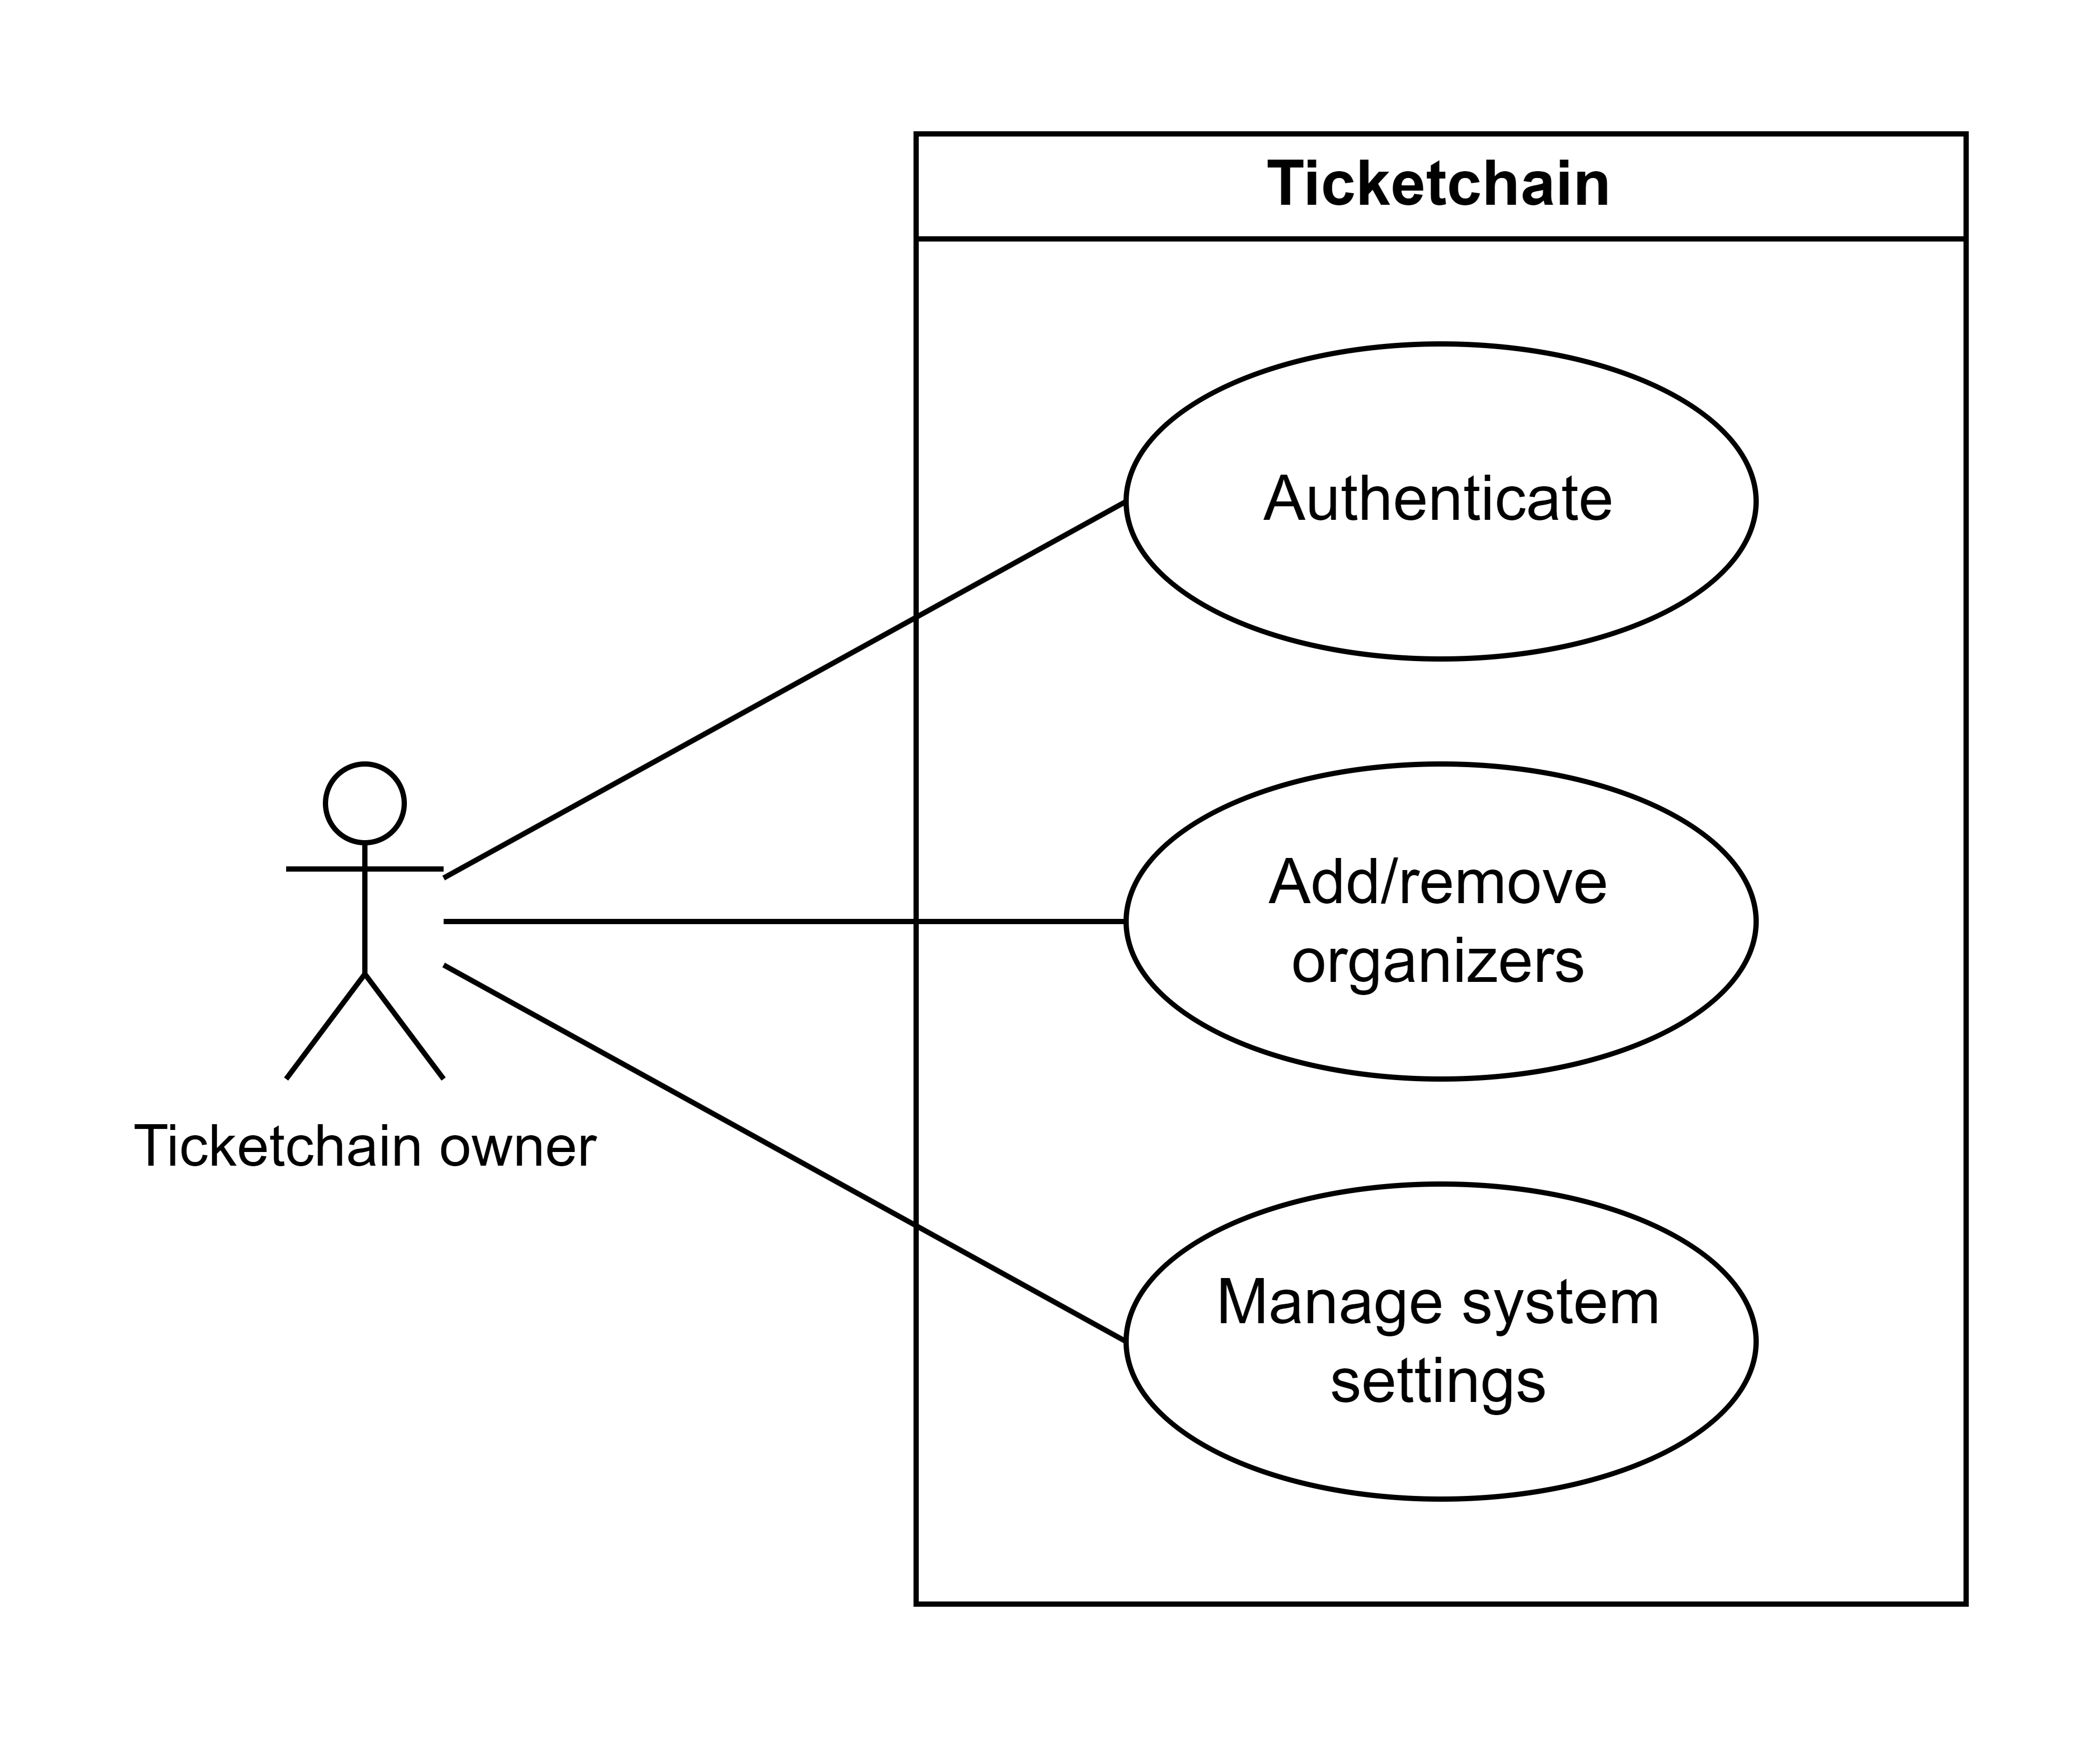
\includegraphics[width=0.5\textwidth]{Ticketchain owner use cases.png}
    \caption{Ticketchain Owner Use Cases}
    \label{fig:ticketchain_owner_use_cases}
\end{figure}

\subsection{Organizer}
\label{subsec:organizer}

As shown in Figure \ref{fig:organizer}, the organizer has several key use
cases, including event creation and management. The organizer also oversees the
selection of validators for each event, ensuring that only authorized personnel
can validate tickets. Furthermore, the organizer can manage event settings,
such as updating information or canceling events when necessary.

\begin{figure}[H]
    \centering
    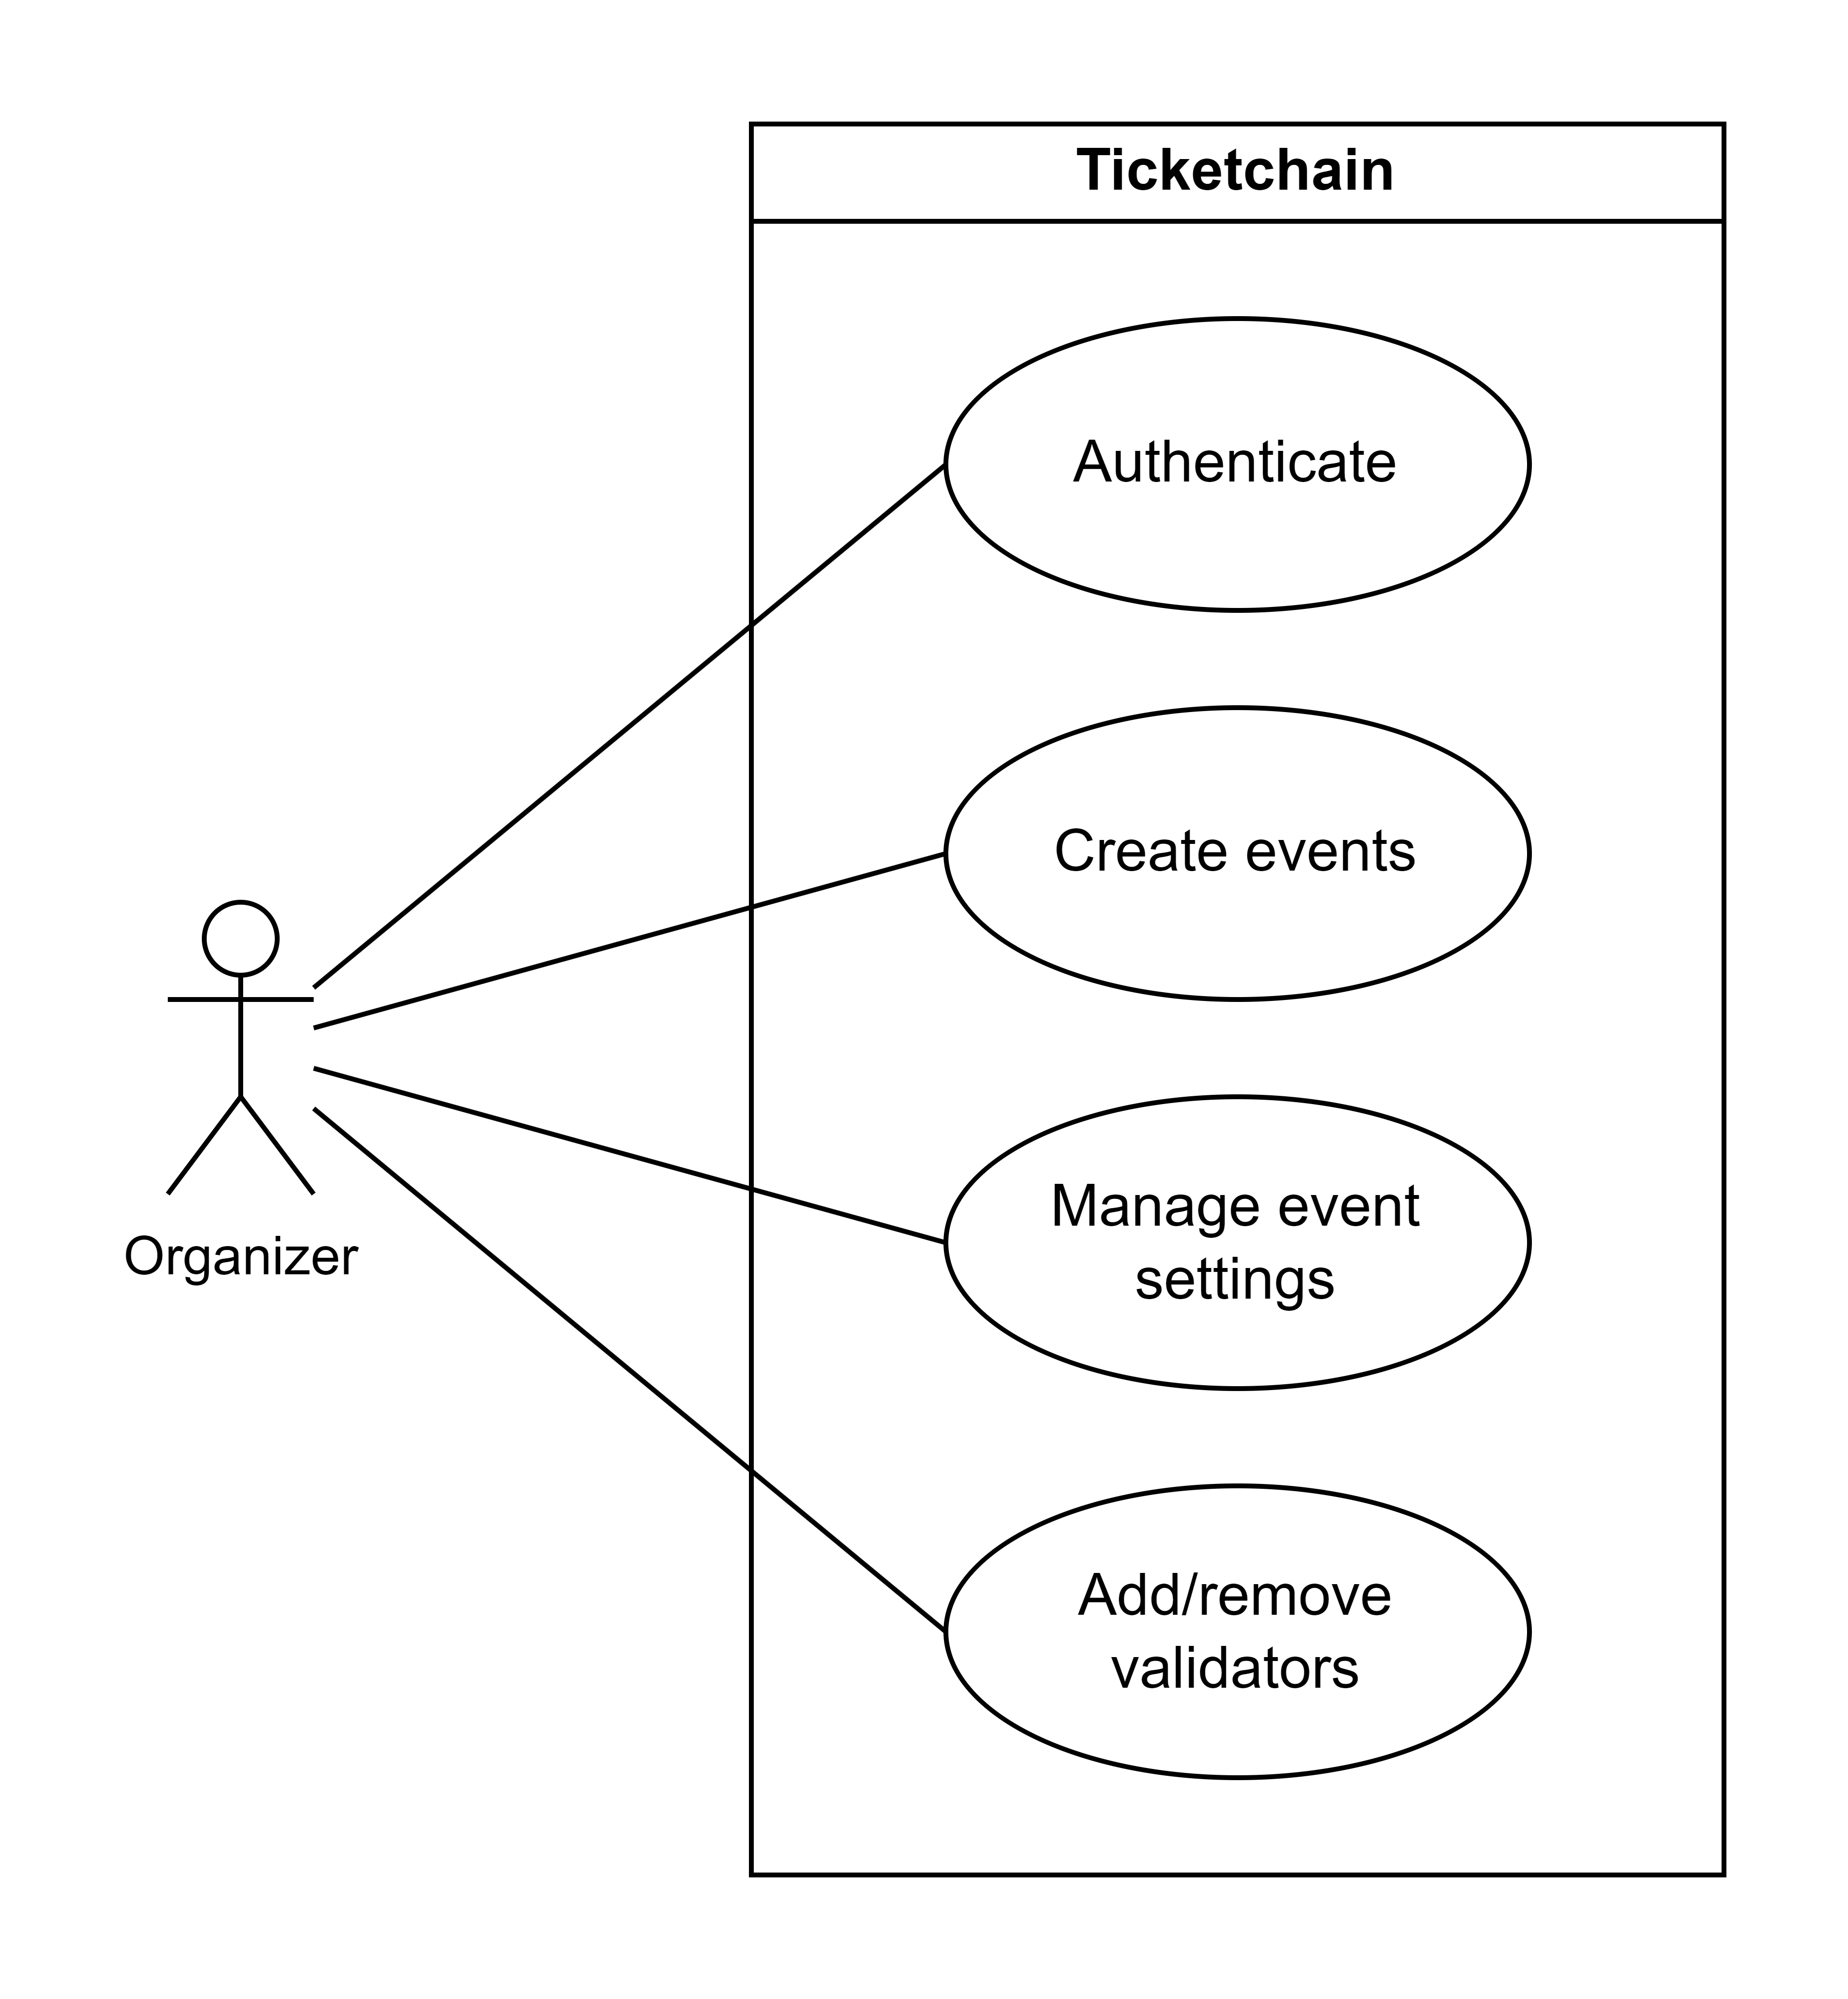
\includegraphics[width=0.5\textwidth]{Organizer use cases.png}
    \caption{Organizer Use Cases}
    \label{fig:organizer_use_cases}
\end{figure}

\subsection{Validator}
\label{subsec:validator}

For validators, as illustrated in Figure \ref{fig:validator_use_cases}, the
primary use case is to validate users' tickets, allowing entry to the event.
This step is critical for maintaining security and ensuring that only users
with valid tickets can participate.

\begin{figure}[H]
    \centering
    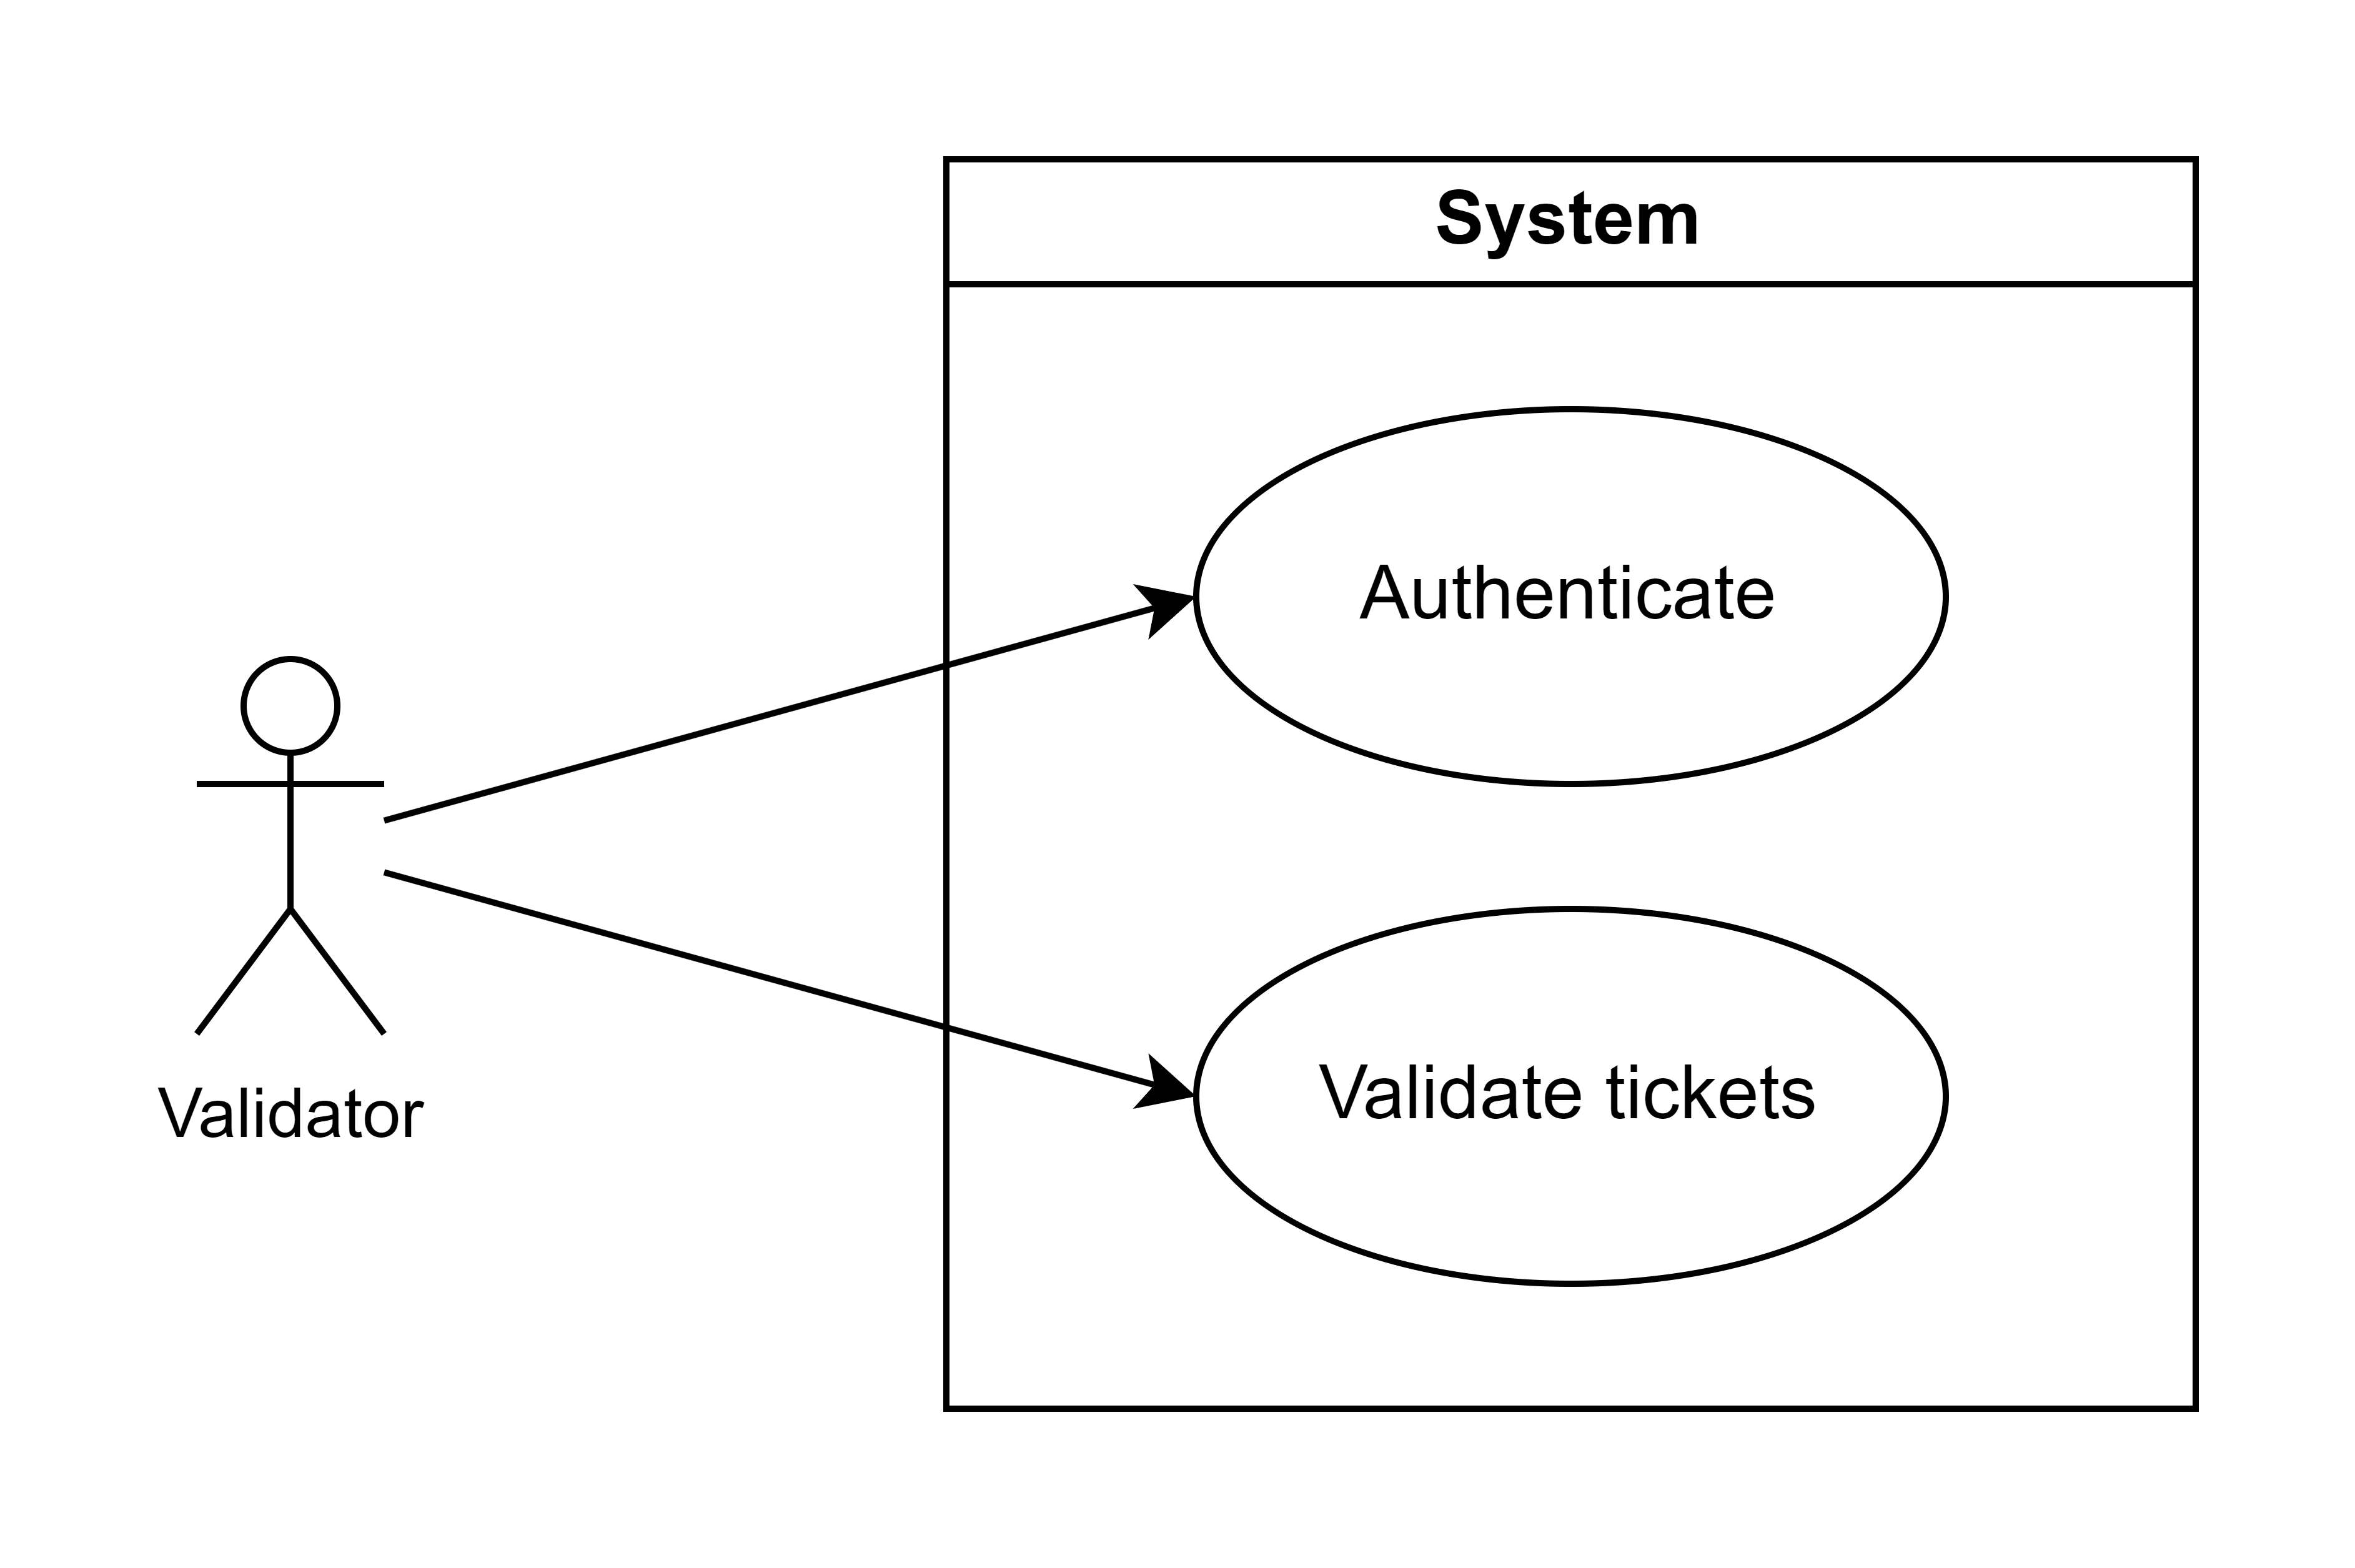
\includegraphics[width=0.5\textwidth]{Validator use cases.png}
    \caption{Validator Use Cases}
    \label{fig:validator_use_cases}
\end{figure}

\subsection{User}
\label{subsec:user}

Figure \ref{fig:user_use_cases} presents the use cases for common users. Users
can purchase tickets, gift them to others, request refunds (depending on event
policies), and resell tickets (with the condition that they cannot sell at a
price higher than the original). These use cases provide users with the
flexibility to manage their tickets according to their preferences while
adhering to system regulations.

\begin{figure}[H]
    \centering
    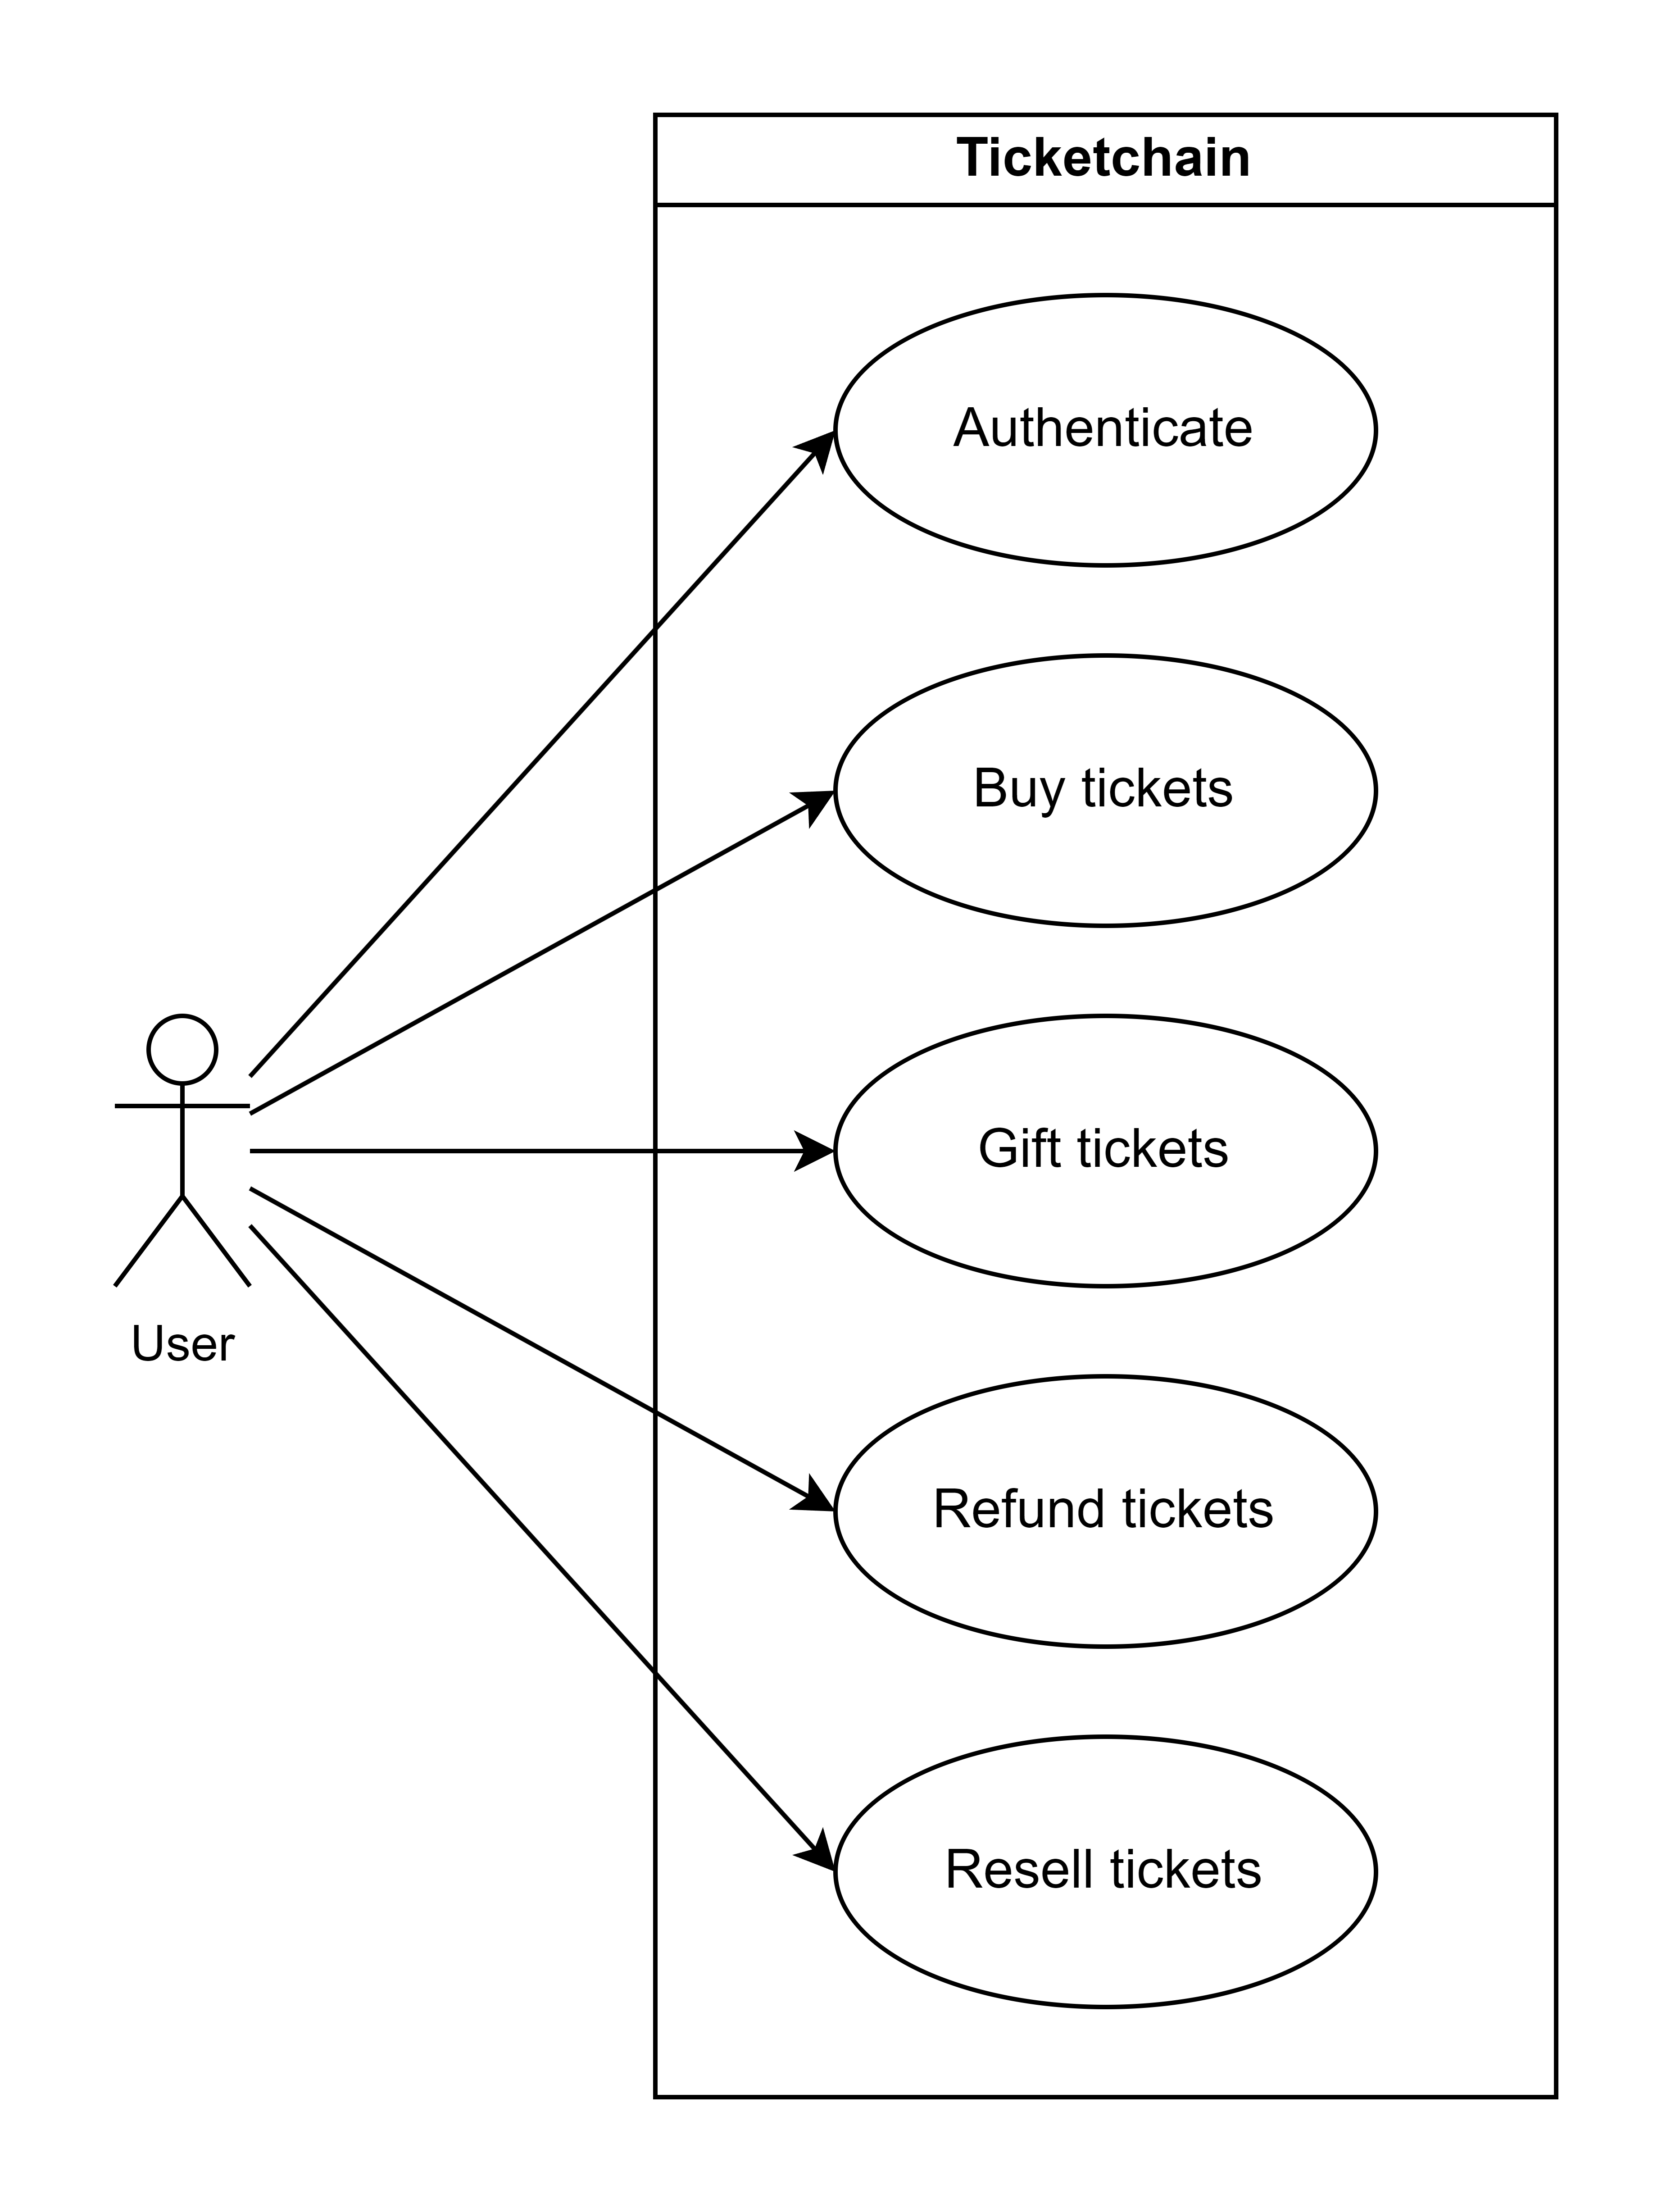
\includegraphics[width=0.5\textwidth]{User use cases.png}
    \caption{User Use Cases}
    \label{fig:user_use_cases}
\end{figure}
